 %!TeX root = Chapter_SignalAnalysis
\documentclass[../../CompleteThesis/Complete_1stDraft]{subfiles}

\begin{document}
The data obtained through various experimental measurements are easily compared with a time series, as they typically show some quantity measured all along the depth of an ice core. This depth is often, at short intervals, treated as a regular linear time series thus making it possible to use some of the known signal analysis methods. Of course, when considering the entirety of an ice core, the linearity disappears as thinning and compression makes the depth series non linear. But when considering short lengths of core it is possible to estimate a linearity, assuming conformity in this specific layer. 

\section[Synthetic Data]{Diffusion Illustrated through Synthetic Data}
\label{Sec:SignalAnalysis_SyntheticData}
\todo{SIGNAL-SYNTHDATA: Write about synthetic data generation.}

\begin{figure}[h]
	\centering
	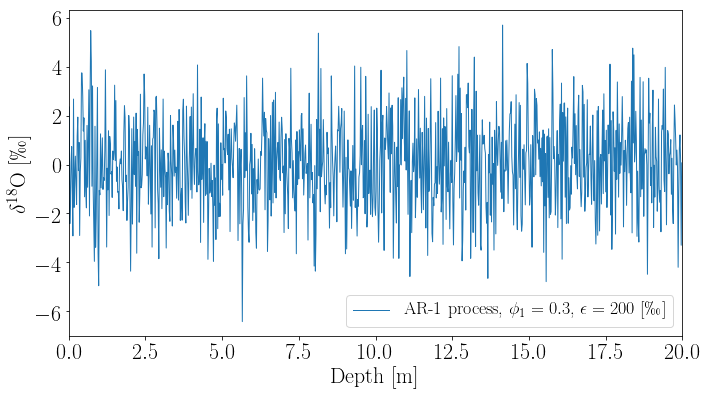
\includegraphics[width=0.8\textwidth]{AR1_process.png}
	\caption[]{}
	\label{fig:AR1_process}
\end{figure}

\begin{figure}[h]
	\centering
	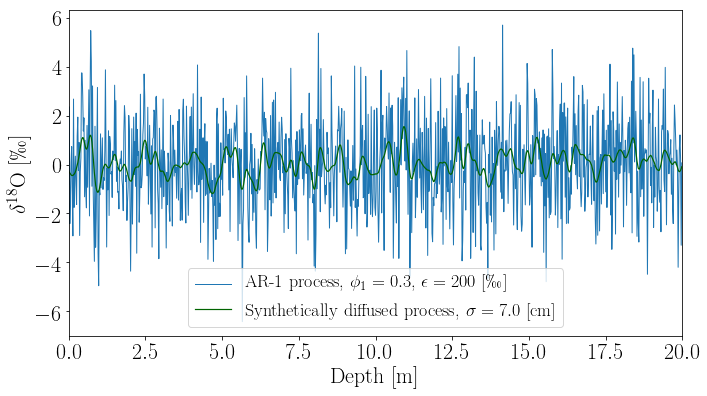
\includegraphics[width=0.8\textwidth]{AR1_process_W_backDiff.png}
	\caption[]{}
	\label{fig:AR1_process_W_backDiff}
\end{figure}

\begin{figure}[h]
	\centering
	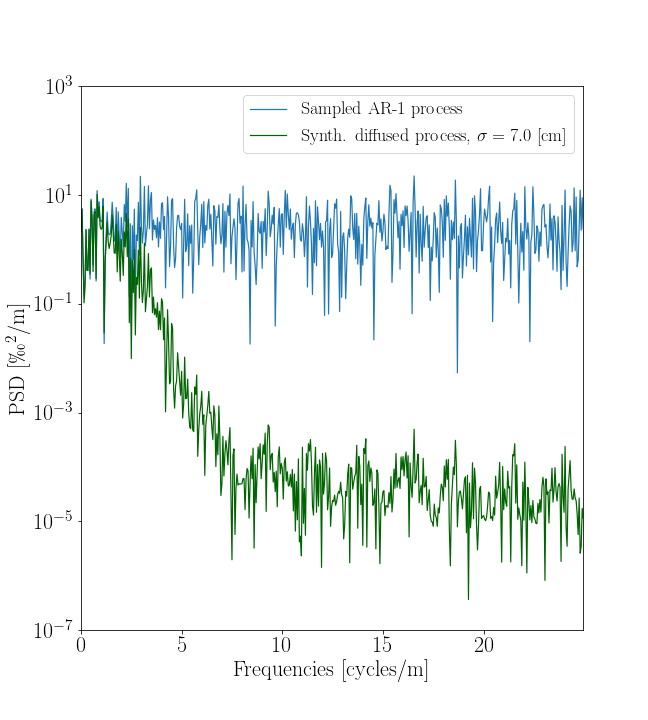
\includegraphics[width=0.6\textwidth]{AR1_process_W_backDiff_PSD.png}
	\caption[]{}
	\label{fig:AR1_process_W_backDiff_PSD}
\end{figure}








\section[Back Diffusion][Back Diffusion]{Back Diffusion}
\label{Sec:SignalAnalysis_BackDiffusion}
Due to diffusion in firn and ice, some of the water isotopic signal is lost. Some of this signal can be restored by investigating the diffusion process, and through filtering and deconvolution techniques(REFERENCES).
For the data of this thesis two different restoration techniques are presented: a spectral method, determining the effect of mixing and diffusion as a spectral filter(REFERENCES), and a kernel restoration method much like the ones used to restore pixel resolution in images (REFERENCES). 
\subsection[Spectral Analysis][Spectral Analysis]{Spectral Analysis}
\label{Subsec:SignalAnalysis_BackDiffusion_SpectralAnalysis}
\subsubsection[PSD][PSD]{Power Spectral Densities}
\label{Subsubsec:SignalAnalysis_BackDiffusion_SpectralAnalysis_PSD}
A very useful tool for analyzing signals exhibiting oscillatory effects is analysis of the signals power spectrum. Instead of considering the signal in time, it is transformed to the spectral domain, where it is possible to obtain an estimate of both the signal and the underlying noise. This is crucial for enhancing the signal and filtering away noise. But to be able to examine these effects, first the data must be transformed. A range of different methods may be used to compute the frequency transform of the depth series, here I present the three I have been working with. Since the data are discrete and experimental, I will be presenting the discrete and applicable mathematical models.\\
When considering a signal, it may be of interest to investigate how the energy of said signal is distributed with frequency. The total power is defined as:
\begin{equation}
	\text{Total Power} = \int_{-\infty}^{\infty} |X(\tau)|^2 \, d\tau.
	\label{Eq:SignalEnergy}
\end{equation}
Using Parseval's theorem (REFERENCE) (assuming that the signal has a finite total energy), the power of the signal can alternatively be written as

\begin{equation}
	\int_{-\infty}^{\infty} |X(\tau)|^2 \, d\tau = \int_{-\infty}^{\infty} |\tilde{X}(\tau)|^2\, df
	\label{Eq:ParsevalsTheorem}
\end{equation}
where $\tilde{X}(f)$ is the spectral (Fourier) transform of the signal, from time to frequency domain, defined as:
\begin{equation}
	\tilde{X}(f) = \int_{-\infty}^{\infty} X(\tau) e^{2\pi i f \tau} \, d\tau
	\label{Eq:FourierTransform}
\end{equation}
and the inverse spectral (Fourier) transform, from frequency to time domain, defined as:
\begin{equation}
	X(t) = \int_{-\infty}^{\infty} \tilde{X}(f) e^{-2\pi i f \tau}\, df.
	\label{Eq:InverseFourierTransform}
\end{equation}
Both $X(t)$ and $\tilde{X}(f)$ represent the same function, just in different variable domains. Often, the angular frequency $\omega$ is used instead, with the relation between $\omega$ and $f$ being $\omega \equiv 2\pi f $, giving the Fourier and inverse Fourier transforms as:

\begin{equation}
	\begin{aligned}
		\tilde{X}(\omega) &= \int_{-\infty}^{\infty} X(t) e^{i\omega\tau}\, d\tau \\
		X(\tau) &= \int_{-\infty}^{\infty} \tilde{X}(\omega) e^{-i\omega\tau}\, d\omega
		\label{Eq:FourierTransformAngular}
	\end{aligned} 
\end{equation}

From Equation \ref{Eq:ParsevalsTheorem} we can interpret the integrand on the right hand side $|\tilde{X}(f)|^2$ as a density function, describing the energy per unit frequency. This is a property which is able to reveal much information about the considered signal, and it is useful to define this as the (one-sided) Power Spectral Density: 
\begin{equation}
	P_X(f) \equiv |\tilde{X}(f)|^2 + |\tilde{X}(-f)|^2 \qquad 0 \leq f < \infty
\end{equation}
This entity ensures that the total power is found just by integrating over $P_X(f)$ from 0 to $\infty$. When the function is purely real, the PSD reduces to $P_X(f) = 2|\tilde{X}(f)|^2$.\\
In the above the transform used to define the PSD was presented as the Fourier transform. When working with discrete data, as is very common when analyzing real world data, there are a number of different ways of estimating the PSD. In the following three different methods will be presented, all used in this thesis.
\newline
\todo{SIGNAL-BACKDIFF: RETHINK THIS PART. DO NOT USE TIME ON ALL THE CALCULATIONS. WRITE THE GENERAL IDEAS OF THE METHODS AND STATE HOW TO CALCULATE/COMPUTE. SMALL CODE SNIP TO GIVE GENERAL IDEA.}
\begin{quote}
	\textcolor{red}{\textbf{RETHINK THIS PART. DO NOT USE TIME ON ALL THE CALCULATIONS. WRITE THE GENERAL IDEAS OF THE METHODS AND STATE HOW TO CALCULATE/COMPUTE. SMALL CODE SNIP TO GIVE GENERAL IDEA.}}
\end{quote}

\subsubsection[DFT \& FFT][DFT \& FFT]{Discrete and Fast Fourier Transform}
\label{Subsubsec:SignalAnalysis_BackDiffusion_SpectralAnalysis_DFTFFT}
The definition of the continuous Fourier transform and its inverse was presented in the above. The Fourier transform is as seen a way of representing the function under consideration as an infinite sum of periodic components. When the function is discrete, so will the Fourier transform be, and the integral is replaced with a sum. This gives us the Discrete Fourier Transform (DFT) which transforms the signal into a sum of separate components contributing at different frequencies. The DFT is dependent on the sampling interval, $\Delta$, and we can describe our discrete signal $X$ as a function of N discrete time steps $t_k = k\cdot\Delta$, where $k = 0, \, 1,\, ..., \, N-1$:
\begin{equation}
	X_k \equiv X(t_k)
	\label{Eq:DiscreteSignal}
\end{equation}
This sample size is supposed to be representative for the entire discrete function, if the function continues beyond the $N$ sampled points. When sampling discretely at interval $\Delta$, there will be a special frequency, the Nyquist critical frequency, defined through the sampling size as:
\begin{equation}
	f_{NQ} \equiv \frac{1}{2\Delta}.
	\label{Eq:NyquistFreq}
\end{equation}
This frequency is of great importance in transformation of discrete signals. If the continuous signal is sampled at an interval $\Delta$ is bandwidth limited to frequencies smaller in magnitude than $f_{NQ}$, $\tilde{X}(f) = 0 \text{ for } |f| \geq f_{NQ}$ - i.e. the transformed function has only non-zero values inside the Nyquist interval, $\tilde{X}(-f_{NQ}), ..., \tilde{X}(f), ..., \tilde{X}(f_{NQ})$. This means that the function is completely determined since we have all information about the signal contained in our available frequency space.\\
On the other hand, which is much more likely, if the continuous signal consists of frequencies both inside and outside the Nyquist interval, then all spectral information outside of this range will be falsely interpreted as being inside this range. Thus a wave inside the interval with a frequency of $f_n$ will have a number of wave siblings outside of the interval, with frequencies  of $k\cdot \frac{1}{\Delta} f_n$, $k$ being integers, which will be aliased into the Nyquist interval and give rise to an increased power at the frequency $f_n$.\\
When analyzing an already measured discrete signal, this might give rise to some headache. What can be done is to assume that the signal has been sampled competently and then assume that the Fourier transform is zero outside of the Nyquist interval. After the analysis it will then be possible to determine if the signal was indeed competently sampled, as the Fourier series will go to zero at $f_{NQ}$ given a correct assumption, and go to a fixed value, if the sampling was not done competently.\\
Now with the basics of understanding the limits of frequency transform of a discretely sampled signal, it is possible to estimate the DFT of the signal $X_k \equiv X(t_k)$. Since the Fourier transform is a symmetric transformation it is easiest to assume that $N$ is even.

Since the input information is of size $N$ we should expect only to sample the frequency transform $\tilde{X}(f)$ at only discrete values of f in the range between the upper and lower critical Nyquist frequencies, $-f_{NQ}$ to $f_{NQ}$:
\begin{equation}
	f_n \equiv \frac{n}{N\Delta}, \qquad n = -\frac{N}{2}, ..., \frac{N}{2}
	\label{Eq:FreqNQRange}
\end{equation}
This will indeed actually give rise to $N+1$ values, since 0 will be in the interval as well, but the limit frequencies are actually not independent, but all frequencies between are, which reduces it to $N$ samples. \\
Now the integral from Equation \ref{Eq:FourierTransform} needs to be estimated as a sum:
\begin{equation}
	\tilde{X}(f_n) = \int_{-\infty}^{\infty} X(\tau) e^{2\pi i f_n \tau} dt \approx  \sum_{k=0}^{N-1}X_k e^{2\pi i f_n t_k} \Delta = \Delta \sum_{k=0}^{N-1}X_k e^{2\pi i k \frac{n}{N}}
	\label{Eq:DFTestimation}
\end{equation}
The Discrete Fourier Transform is thus defined as:
\begin{equation}
	\tilde{X}_n \equiv  \sum_{k=0}^{N-1}X_k e^{2\pi i k \frac{n}{N}}
	\label{Eq:DFT}
\end{equation}
This gives the approximate relation between the DFT estimate and the continuous Fourier transform $\tilde{X}(f)$ when sampling at size $\Delta$ as:
\begin{equation}
	\tilde{X}(f_n) \approx \Delta \tilde{X}_n
\end{equation}
The inverse DFT is given as:
\begin{equation}
	X_n \equiv \frac{1}{N} \sum_{n=0}^{N-1}X\tilde{X}_n e^{-2\pi i k \frac{n}{N}}
	\label{Eq:InverseDFT}
\end{equation}
Computation of the DFT can be very slow and tiresome, since it involves complex multiplication between a number of vectors and matrices. If we write Equation \ref{Eq:DFT} as $\tilde{X}_n = \sum_{k=0}{N-1}W^{nk}X_k,$ where  $W$ is a complex number $W\equiv e^{2\pi i /N}$. This shows that the vector $X_k$ must be multiplied with a complex matrix which (n,k)th component consists of the constant $W$ to the power of $nk$. This matrix multiplication evidently leads to a process of $O(N^2)$. Fortunately, a number of different algorithms implementing a wide range of different theories from complex number arithmetic and prime-factoring to group and number theory (\cite{Cooley1965},\cite{Good1958_PrimeFFT}, \cite{Bruun1978__BruunsFFT} and others) have been developed for fast and efficient computation of the discrete Fourier transform. One of these is called the Fast Fourier Transform (FFT), which can reduce the computations to just $\mathcal{O}(N\log_2 N)$. In this thesis the FFT used is the one implemented in the \lstinline[language=Python]|scipy.fft| Python package \cite{Virtanen2020_SciPy}, which is based on the works of \cite{Cooley1965}. See said article for implementation details. One important thing about this specific algorithm is that for the algorithm to function most efficiently, the number of points computed in the frequency space must be of a power of 2, following the use of base $\log_2$

\subsubsection[NUFT][NUFT]{Nonuniform Discrete Fourier Transform}
\label{Subsubsec:SignalAnalysis_BackDiffusion_SpectralAnalysis_NUFT}
All FFT algorithms evaluates the DFT definitions from Eqs. \ref{Eq:DFT} to \ref{Eq:InverseDFT} in fast and efficient ways. But one key assumption for these methods is that the data under examination are equispaced, i.e. uniformly distributed, based on the summation in Eq. \ref{Eq:DFT}. The computations thus expect uniform data as input and returns uniform data as output. Unfortunately this is not always the case for data collected in physical experiments. In this case the basic assumptions for the calculations of both DFT and FFT are flawed. \\
The most general form of a nonuniform transform would be the one that takes non-equispaced data as input and also returns non-equispaced transforms as output. Firstly we wish to create a nonuniform discrete Fourier transform (NUDFT) that transforms a sequence of $N$ complex numbers $X_0,...,X_{N-1}$ to a different sequence of $M$ complex numbers, $\tilde{X}_0,...,\tilde{X}_{M-1}$. The one-dimensional NUDFT the computes the transformed vector $\tilde{\boldsymbol{X}} = (\tilde{X}_0,...,\tilde{X}_{M-1})^{\text{T}}$, with entries computed as the sum
\begin{equation}
	\tilde{X}_k = \sum_{n=0}^{N-1} X_n e^{-2\pi i p_n f_k},\qquad 0 \leq k \leq M-1.
	\label{Eq:NDFT} 
\end{equation}
The values $X_0, ...,X_{N-1}$ are sample values, $p_0,...,p_{N-1}$ are sample positions and $f_0,...,f_{M-1}$ are frequencies. The NUDFT vector $\tilde{\boldsymbol{X}}$ is found by computing $M$ sums with each $N$ terms. This meaning that the computational cost will be of order $\mathcal{O}(M\cdot N)$, and if $M=N$ then of $\mathcal{O}(N^2)$. The NUDFT reduces to the DFT if the points are equispaced, $p_n = \frac{n}{N}$, and the frequencies are integers, $f_k = k$, and can be computed at the cost of the FFT, $\mathcal{O}(N\log_2 N)$. In the literature there are many who have presented different ways to develop a fast NUDFT (\cite{Potts2001}, \cite{Marvasti1993}, \cite{Ruiz-Antolin2018}, \cite{Lee2005} among others), generally referred to as NUFFT or NFFT. In this work though, the main focus is on the discrete cosine transform, and the NFFT methods will not be described in depth\\


\subsubsection[DCT][DCT]{Discrete Cosine Transform}
\label{Subsubsec:SignalAnalysis_BackDiffusion_SpectralAnalysis_DCT}
The Fourier transform in any of its many forms is designed to process complex-valued signals, always producing a complex-valued spectrum, even for signals that were strictly real-valued. The real-valued or complex-valued part of the Fourier spectrum is on their own not enough to represent the full information of the signal, since neither the cosine nor he sine functions (corresponding to the real and the complex parts of the spectrum respectively), constitute a complete set of basis functions. Nonetheless, a purely real-valued signal has a symmetric Fourier spectrum, meaning that it is only necessary to compute half the number of spectral coefficients, without losing any signal information. Since the signals analyzed in this thesis are strictly real, one way to use this knowledge to improve on the works of this project is to consider a different, less expensive, purely real spectral transform. The cosine transform \cite{Ahmed1974_DCT} seems to do the trick: it uses only cosine functions as basis functions and operates with only real-valued signal and spectral coefficients, and have properties similar to the Fourier transform.\\
For the discrete version of the cosine transform, DCT, and its inverse, IDCT, a number of different definitions have been proposed, but for this work, the originally formulations by \cite{Ahmed1974_DCT} are used. These are often referred to as "The DCT" and "The IDCT", and other times as DCT-II and DCT-III. The entries of the computed discrete cosine transform vector,$\tilde{X}_0,...,\tilde{X}_{M-1}$ , of a real-valued signal of $N$ data points, $X_0,...X_{N-1}$, is computed as
\begin{equation}
	\tilde{X}_k = 2\sum_{n=0}^{N-1} X_n \cos\left(\frac{\pi(2n+1)k}{2N}\right),\qquad 0\leq k < M.
	\label{Eq:DCT}
\end{equation}

To orthonormalize the base functions,$\phi_k(n)$ , the coefficients are multiplied by a scaling factor $f$:
\begin{equation}
	f = \begin{cases}
		\frac{1}{\sqrt{2N}}, & \text{if} k = 0 \\
		\frac{1}{\sqrt{4N}}, & \text{otherwise}
	\end{cases}
	\label{Eq:DCT_OrthoScalingFactor}
\end{equation}
so that the base functions, $\phi_k[n] = 2f\cos\left(\frac{\pi(2n+1)k}{2N}\right)$, meet the condition:
\begin{equation}
	\sum_{n=0}^{N-1} \phi_k[n]\phi_l[n] = \delta_{lk}.
	\label{Eq:DCT_Orthonormalization}
\end{equation}

The inverse of the DCT, the so called DCT-III, is defined, unnormalized, as: 
\begin{equation}
	X_k = \tilde{X}_0 + 2\sum_{n=1}^{N-1} \tilde{X}_n\cos\left(\frac{\pi n(2k+1)}{2N}\right), \qquad 0 \leq k < N 
	\label{Eq:IDCT}
\end{equation}
and orthonormalized:
\begin{equation}
	X_k = \frac{\tilde{X}_0}{\sqrt{N}} + \sqrt{\frac{2}{N}}\sum_{n=1}^{N-1} \tilde{X}_n\cos\left(\frac{\pi n(2k+1)}{2N}\right), \qquad 0 \leq k < N 
	\label{Eq:IDCT_ortho}
\end{equation}

Only when the DCT-III is orthonormalized is it exactly the inverse of the orthonormalized DCT-II. If they are both unnormalized, the DCT-III is the inverse of the DCT-II up to a factor $2N$.
As with the DFT, the DCT can directly be computed at a cost of $\mathcal{O}(N\cdot M)$, and can also reduced to $\mathcal{O}(N \log N)$. The fast DCT algorithm(FCT) used here is based on \cite{Makhoul1980} as it is implemented in the \lstinline[language=Python]|scipy.fft.dct| package\cite{Virtanen2020_SciPy}.

\subsubsection[NDCT][NDCT]{Nonuniform Discrete Cosine Transform}
\label{Subsubsec:SignalAnalysis_BackDiffusion_SpectralAnalysis_NDCT}
Again, as with the FFT, the FCT works under the key assumption that data is equispaced. Though when data is nonuniform, the DCT is described as:
\begin{equation}
	\tilde{X}_k = 2\sum_{n=0}^{N-1}X_n \cos\left(2\pi f_k\left(p_n + \frac{1}{2N}\right)\right), \qquad 0 \leq k < M-1
	\label{Eq:NDCT}
\end{equation}
with, in the most general case, nonuniformly spaced signal, $p_o,...,p_{N-1}$, data and frequency data, $f_0,...,f_{M-1}$.
The inverse of NDCT, the INDCT, is computed as:
\begin{equation}
	X_k = \frac{\tilde{X}_0}{\sqrt{N}} + \sqrt{\frac{2}{N}}\sum_{n=1}^{N-1} \tilde{X}_n \cos\left(\left(p_n + \frac{1}{2N}\right)2\pi f_k\right), \qquad 0 \leq k < N -1
	\label{Eq:INDCT}
\end{equation}

It is possible to develop algorithms with the computational cost of $\mathcal{O}(N\log N)$ for NDCT and INDCT as it is for 
the NDFT (\cite{Tian2000}, \cite{Zhao2008}) but it has showed to be out of the scope of this project and has not been implemented. This of course slows down the final optimization algorithm, as it requires a number of spectral transformations. In Section \ref{Sec:Method} it is described how the final algorithm has been designed to minimize the use of NDCT, and thus speeding up the final computations.

\begin{figure}
	\centering
	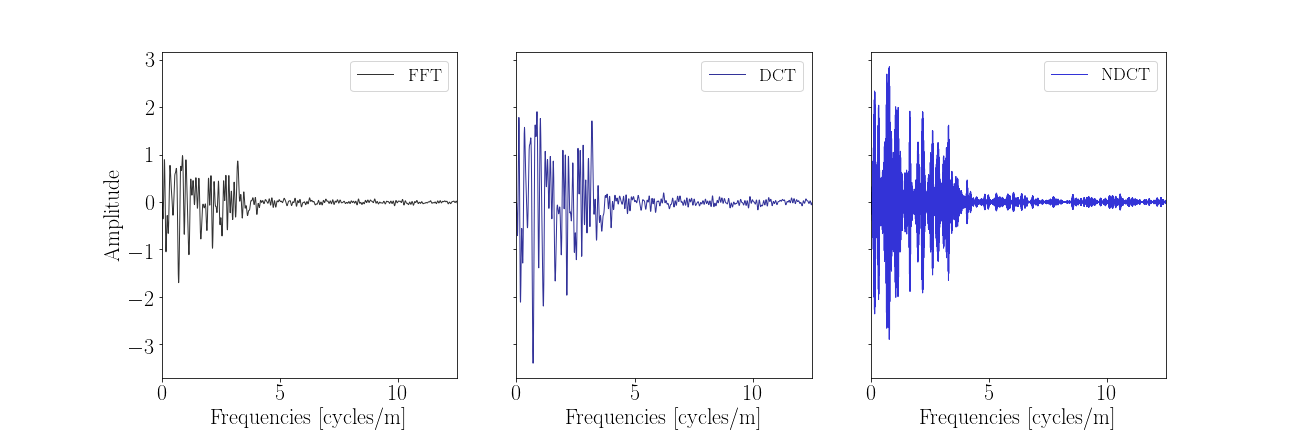
\includegraphics[width=\textwidth]{SpectralTransforms_3.png}
	\caption[FFT, DCT, NDCT, Site A]{Examples of three different spectral transforms, FFT, DCT, NDCT, performed on the depth series between Tambora and Laki eruptions from Site A.}
	\label{fig:SpectralTransforms_3}
\end{figure}

\begin{figure}
	\centering
	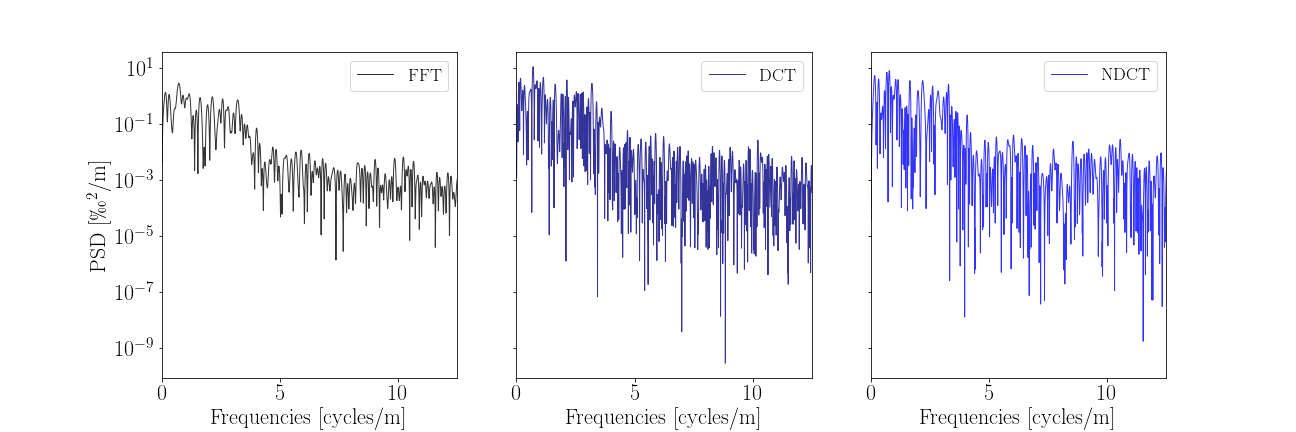
\includegraphics[width=\textwidth]{SpectralTransforms_PSD.png}
	\caption[FFT, DCT, NDCT PSDs, Site A]{Examples of power spectral densities related to the three different spectral transforms, FFT, DCT, NDCT, seen in Figure \ref{fig:SpectralTransforms_3}.}
	\label{fig:SpectralTransforms_PSD}
\end{figure}



\subsubsection[MEM][MEM]{Maximum Entropy Method (Burg's Method)}
\label{Subsubsec:SignalAnalysis_BackDiffusion_SpectralAnalysis_MEM}
\todo{SIGNAL-MEM: Write this entire section - maybe not necessary? Maybe use in reconstruction of missing data...}

\subsection[Spectral Filtering][Spectral Filtering]{Spectral Filtering}
\label{Subsec:SignalAnalysis_BackDiffusion_SpectralFiltering}
\subsubsection[Wiener Filtering][Wiener Filtering]{Wiener Filtering}
\label{Subsubsec:SignalAnalysis_BackDiffusion_SpectralFiltering_Wiener}
Through spectral analysis it is possible to treat the noise of the signal consistently. The goal is to create spectral filters which enhances the signal while minimizing the effect of the noise, thus increasing the signal-to-noise ratio (SNR).\\
Theoretically, without any diffusion, the change in isotopic concentration would be described through a step function, going from one constant concentration to another. This step function can be described by the Heaviside function:
\begin{equation}
	D(t) = \begin{cases}
		0, & t < 0 \\
		1, & t \geq
	\end{cases}
\end{equation}
In reality, a number of different mixing processes change this step function, and the measured signal will be a smooth curve, $s(t)$, which corresponds to the convolution of $S(t)$ with the mixing response function $M(\tau)$
\begin{equation}
	d(t) = \int_{- \infty}^{\infty} D(\tau) \cdot M(t - \tau)d\tau
\end{equation}


\subsection[Signal Restoration][Signal Restoration]{Signal Restoration by Optimal Diffusion Length}
\label{Subsec:SignalAnalysis_BackDiffusion_SignalRestoration}
\subsubsection{Kernel Estimation}
\label{Subsubsec:SignalAnalysis_BackDiffusion_SignalRestoration_KernelEstimation}
As is well known, in the spectral domain, convolution is multiplication and the mixing is described as the multiplication between the Fourier transform of $S$ and $M$:
\begin{equation}
	\tilde{d} = \tilde{D} \cdot \tilde{M}
\end{equation}


By differentiation with respect to time, the mixing filter $M$ is unaffected, and differentiation of the measured system response, the Heaviside function, $S'$ is a delta function, which Fourier transformed is unity, leading to:
\begin{equation}
	\tilde{d'} = \tilde{D'} \cdot \tilde{M} = \tilde{M}
\end{equation}
The mixing filter can thus be determined by measuring the system response to a step function, differentiating performing Fourier transform of the result $d'$.

After determination of the mixing filter $\tilde{M}$, the unmixed signal $D$ can be estimated in theory by inverse Fourier transform of


\begin{equation}
	\tilde{D} = \tilde{d}\cdot\tilde{M}^{-1}
	\label{eq:Restoration}
\end{equation}

During the mixing, cycles with short wavelengths are heavily washed out, and through the restoration in Eq. \ref{eq:Restoration}, the amplitudes corresponding to these wavelengths are heavily amplified by the filter. This method though has a drawback, which is that when the measurements contain noise, the restored signal will be dominated by high-frequency noise, greatly amplified by the mixing filter. Thus it is a problem of retaining as much (short wavelength) signal as possible while simultaneously attempting to amplify the high-frequency noise as little as possible. This optimal trade-off can be found by creating an optimum filter for the considered measured isotopic signal:
\begin{equation}
	\delta_M(z) = \delta_m (z) + \eta(z)
\end{equation} 
This optimal (Wiener) filter $\tilde{F}$, defined for each wave number $k = 2\pi \omega$, is presented as the ratio between pure signal and pure signal plus noise described in Power Spectral Densities as:
\begin{equation}
	\tilde{F}(k) =\frac{|\tilde{\delta_m}(\omega)|^2}{|\tilde{\delta_m}(\omega)|^2 + |\tilde{\eta}(\omega)|^2}
	\label{eq:WienerFilter}
\end{equation}
In this work, the power spectral densities of the signal and the noise, respectively, are determined through analysis of the power spectral density of the combined signal/noise PSD.\\
The PSD of the noise free measured signal, $|\tilde{\delta_m}(\omega)|^2$, is assumed describe as 
\begin{equation}
	|\tilde{\delta}_m(\omega)|^2 = P_0 e^{-k^2 \sigma_{\text{tot}}^2}
	\label{eq:SignalPSD}
\end{equation}
where $\sigma_{\text{tot}}^2$ describes the total estimated diffusion length of the mixing.\\
The noise is assumed to be red noise, described by an autoregressive process of first order, AR1:
\begin{equation}
	|\tilde{\eta}(\omega)|^2 = \frac{\sigma_{\eta}^2 \Delta z}{|1 + a_1 \exp(-2\pi i \omega \Delta z)|^2}
	\label{eq:NoisePSD}
\end{equation}
where $\sigma_{\eta}^2$ is the variance of the red noise, $a_1$ is the AR1 coefficient and $\Delta z$ is the resolution of the time/depth data.
It is then possible to estimate the parameters $P_0$, $\sigma_{\text{tot}}^2$, $\sigma_{\eta}^2$ and $a_1$ by curve fitting, separately, the two expressions in Eq. \ref{eq:SignalPSD} and \ref{eq:NoisePSD} to the data. The estimated parameters are varied to find the optimal guess to use for the filter.

\begin{figure}
	\centering
	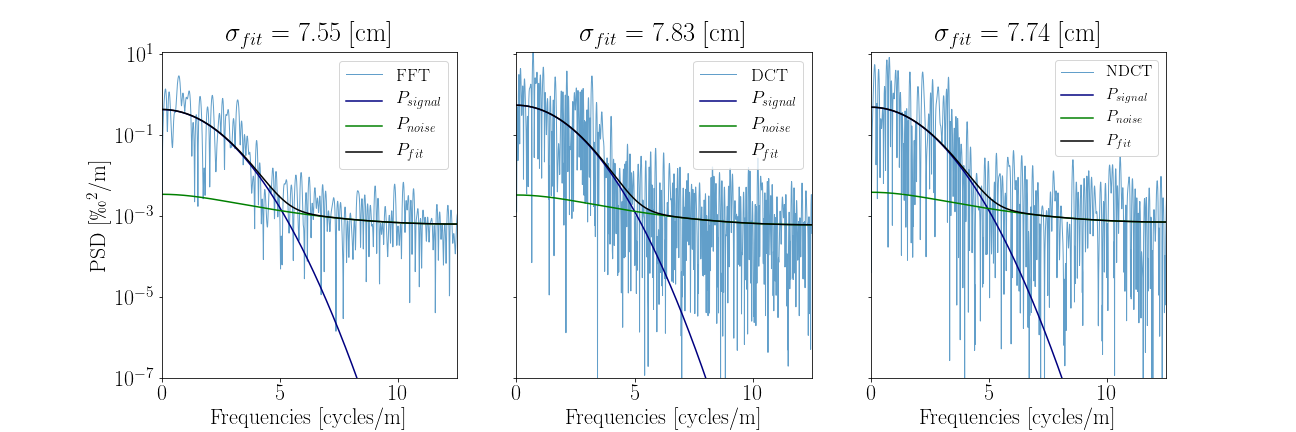
\includegraphics[width=\textwidth]{SpectralTransforms_PSDwFits.png}
	\caption[FFT, DCT, NDCT PSDs with Fit, Site A]{Noise, signal and total fit to PSD, illustrating the construction of the Wiener Filter, see Sec. \ref{Sec:SignalAnalysis_Restoration}.}
	\label{fig:SpectralTransforms_PSDwFits}
\end{figure}


\section[Restoration][Restoration]{Enhanced Resolution and Restoration of Signal}
\label{Sec:SignalAnalysis_Restoration}

\subsection[Interpolation]{Interpolation of Data}
\label{Subsec:SignalAnalysis_Restoration_Interpolation}
For the purpose of this thesis, interpolation of data needs to be fast, efficient and result in a function as smooth as possible. The last criterion is due to the knowledge of the nature of the data. The measurements are not continuous but should indeed in theory be so. Thus a good choice for interpolation of the data examined in this thesis would be the cubic spline interpolation. An instance of a such interpolation can be seen in Figure \ref{fig:Interp}.\\
Cubic spline interpolation has been used in two instances during this analysis, both times through the \lstinline[language=Python]|Python SciPy| package \lstinline[language=Python]|scipy.interpolate.CubicSpline|\todo{SIGNAL-INTERP: REFERENCE!!}. Firstly, to assure equally spaced data points, so as to be able to perform a useful frequency analysis through spectral transformation, see Section, \ref{sec:???}. Secondly cubic spline interpolation was used to improve on peak detection in the final back diffused data. The final data have a rather low resolution, leading to an initial guess of peak positioning that might be shifted due to the discretization. Through cubic spline interpolation it is possible to construct a smooth estimate of a signal of higher resolution, leading to a peak positioning estimate that might be less shifted, see Figure \ref{fig:InterpFinal}.

\subsection[Standardisation]{Detrending and Standardising}
\label{Subsec:SignalAnalysis_Restoration_Standardisation}

\todo{SIGNAL-STANDARD: Think about if this is necessary. Maybe work into recursivity and constraints in Method?}
\subsection[Cycle Length Estimation][Cycle Length Estimation]{Cycle Length Estimation of Detrended Signal}
\label{Subsec:SignalAnalysis_Restoration_CycleLengthEst}
\todo{SIGNAL-CYCLE: Think about if this is necessary. Maybe work into recursivity and constraints in Method?}
	
\end{document}
